\section{Patrones de Diseño Facade} 
\textbf{}\\
\begin{flushleft}
patrones de diseño se consideran una de las herramientas más valiosas para producir diseños de calidad y una técnica de propósito general para mejorar un diseño es identificar todas las realizaciones de patrones y aplicar reglas conocidas para mejorarlos.

\begin{itemize}
	\item Patrones de Diseño
	\\es un tipo de patrón de diseñoestructural. Viene motivado por la necesidad de estructurar un entorno de
programación y reducir su complejidad con la división en subsistemas, minimizando las comunicaciones y dependencias
entre estos.

     \item Consideraciones para su aplicación
  \\Se aplicará el patrón fachada cuando se necesite proporcionar una interfaz simple para un subsistema complejo, o cuando se quiera estructurar varios subsistemas en capas, ya que las fachadas
serían el punto de entrada a cada nivel. Otro escenario proclive para su aplicación surge de la necesidad de desacoplar un sistema de sus clientes y de otros subsistemas, haciéndolo más
independiente, portable y reutilizable (esto es, reduciendo dependencias entre los subsistemas y los clientes).


	


	\item ¿Qué es una fachada o facade en inglés?
	\\ Es un patrón de diseño que nos permite simplificar el interface de comunicación entre dos objetos.

\item Estructura
	\begin{center}
	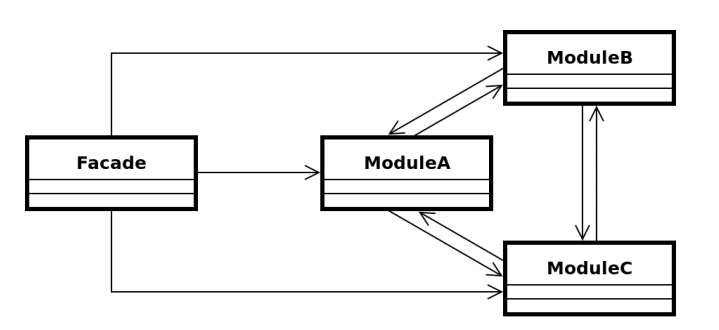
\includegraphics[width=10cm]{./Imagenes/facade1} 
	\end{center}

	
	\begin{center}
	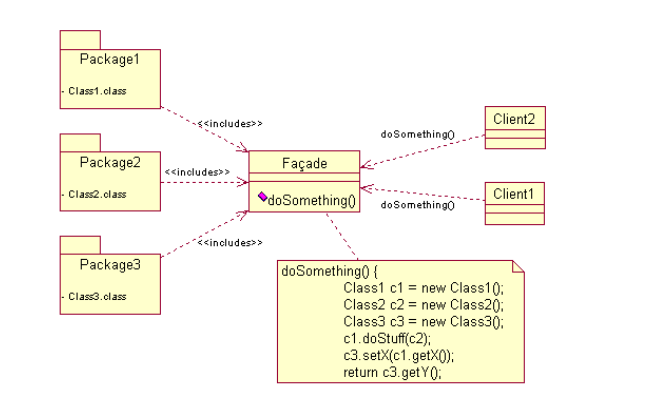
\includegraphics[width=10cm]{./Imagenes/facade2} 
	\end{center}
\item Participantes
\\Fachada (Facade): conoce qué clases del subsistema son responsables de una determinada petición, y delega esas peticiones de los clientes a los objetos apropiados del subsistema.

\item Colaboraciones
\\Los clientes que se comunican con el subsistema enviando peticiones al objeto Fachada, el cual las reenvía a los objetos apropiados del subsistema.
\\Los objetos del subsistema realizan el trabajo final, y la fachada hace algo de trabajo para pasar de su interfaz a las del subsistema.
\\Los clientes que usan la fachada no tienen que acceder directamente a los objetos del subsistema.

\item Ventajas e inconvenientes
\\La principal ventaja del patrón fachada consiste en que para modificar las clases de los subsistemas, sólo hay que realizar cambios en la interfaz/fachada, y los clientes pueden permanecer
ajenos a ello. Además, y como se mencionó anteriormente, los clientes no necesitan conocer las clases que hay tras dicha interfaz.

Busca simplificar el sistema, desde el punto de vista del cliente, proporcionando una interfaz unificada para un conjunto de subsistemas, definiendo una interfaz de nivel más alto. Esto hace que el sistema sea más fácil de usar.

Este patrón busca reducir al mínimo la comunicación y dependencias entre subsistemas. Para ello, utilizaremos una fachada, simplificando la complejidad al cliente. El cliente debería acceder a un subsistema a través del Facade. De esta manera, se estructura un entorno de programación más sencillo, al menos desde el punto de vista del cliente (por ello se llama "fachada").


         \item ¿Se debe utilizar cuando?
	\\ Se quiera proporcionar una interfaz sencilla para un subsistema complejo.
             Se quiera desacoplar un subsistema de sus clientes y de otros subsistemas, haciéndolo más independiente y portable.
            Se quiera dividir los sistemas en niveles: las fachadas serían el punto de entrada a cada nivel. Facade puede ser utilizado a nivel aplicación.
	\begin{center}
	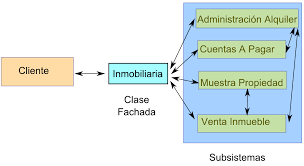
\includegraphics[width=10cm]{./Imagenes/facade3} 
	\end{center}

Los clientes se comunican con el subsistema a través de la facade, que reenvía las peticiones a los objetos del subsistema apropiados y puede realizar también algún trabajo de traducción. Los clientes que usan la facade no necesitan acceder directamente a los objetos del sistema.	
	

\end{itemize} 


\end{flushleft}